José Santos y Ángel Monteagudo realizaron una serie de simulaciones en su artículo
donde intentan estudiar la influencia de los marcadores en la evolución de la simulación.
Todas las simulaciones, y sus resultados, se comentan en esta sección.

El tamaño de rejilla utilizada para todos los experimentos es de $50^3$. Esto son,
$125.000$ células posibles en la rejilla.

\section{Influencia del parámetro \textit{Tasa de mutación base (m)}}

Los autores en su artículo presentan 3 experimentos utilizando los valores por defecto
y variando el parámetro \textit{Tasa de mutación base (m)} para estudiar como afecta
dicho parámetro en la proliferación del cáncer.

Cada experimento se muestra en una serie de gráficas en las cuales se presenta
como resultado la media de 5 ejecuciones diferentes.

A continuación, se muestra cada uno de los experimentos especificando en cada caso
el valor $m$ utilizado. El resto de parámetros de la simulación se mantiene constante
con los valores considerados por defectos, que son:

\begin{table}[h!]
  \centering
  \caption{Valores de los parámetros, excepto \textit{m}.}
  \label{tab:table1}
  \begin{tabular}{ccc}
    \toprule
    Nombre & Símbolo & Valor\\
    \midrule
    Tamaño del telómero & tl & 50\\
    Muerte por daño genético & e & 10\\
    Factor de incremento de tasa de mutación base & i & 100\\
    Muerte de un vecino & g & 30\\
    Muerte aleatoria & a & 1000\\
    \bottomrule
  \end{tabular}
\end{table}

\subsection{Experimento 1: Tasa de mutación base igual a 10.000}

En este primer experimento, los autores presentan un valor para el parámetro
tasa de mutación base de $m=10000$. Realizan una simulación de $1000$ iteraciones.

Es importante recordar, que al utilizar $1/m$ para representar la probabilidad
de que aparezcan diferentes mutaciones al realizar la mitosis, a mayor valor
del parámetro $m$, menor probabilidad de que ocurran mutaciones.

En la simulación, el número de células cancerosas es muy bajo y crece muy levemente,
no superando las $10000$ células de las $125000$ totales. En cuanto a lo marcadores,
el marcador $SG$ toma ventaja y tiene ocurrencia en la mayoría de células cancerosas
(una célula cancerosa es aquella que tiene, al menos, una mutación). El siguiente marcador
presente, aunque con mucha diferencia, es $EA$. El resot de marcadores presenta
un comportamiento similar y su presencia es casi inexistente.

\begin{figure}[h]
\centering
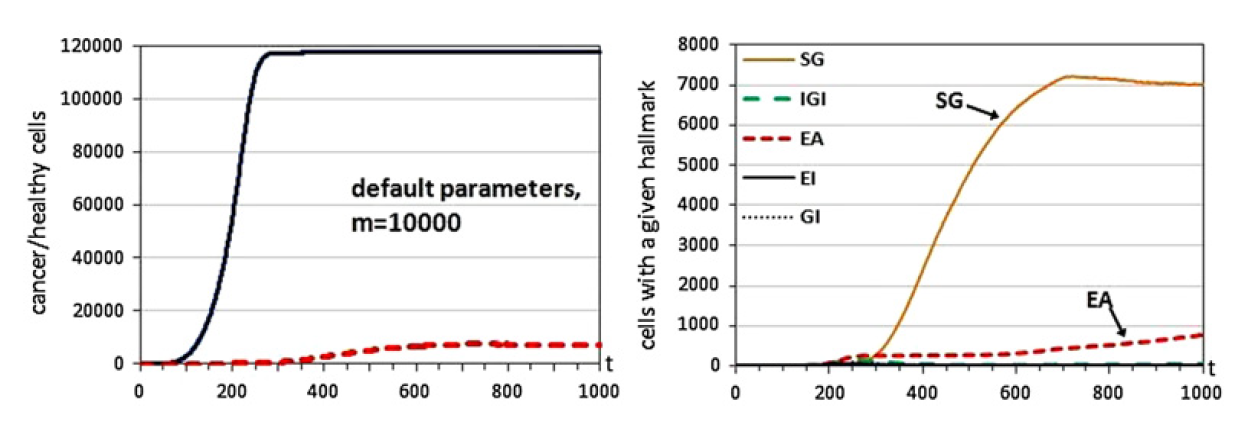
\includegraphics[scale=0.6]{figures/experiments/exp1}
\caption{Resultados obtenidos por los autores para el experimento con $m=10,000$.}
\end{figure}

\subsection{Experimento 2: Tasa de mutación base igual a 1.000}

En el segundo experimento, los autores alteran el valor para el parámetro tasa de
mutación base a $m=1000$.

Los resultados obtenidos para $1000$ iteraciones presentan varias diferencias. En primer lugar,
el número de células cancerosas aumenta, lo cual, se explica por la mayor probabilidad
de mutaciones provocadas al realizar la mitosis. En segundo lugar, en cuanto a los marcadores,
aparecen todos los marcadores, con un comportamiento bastante similar entre ellos. Se pueden
destacar los marcadores $EA$ y $SG$, que toman algo de ventaja respecto al resto.

\begin{figure}[h]
\centering
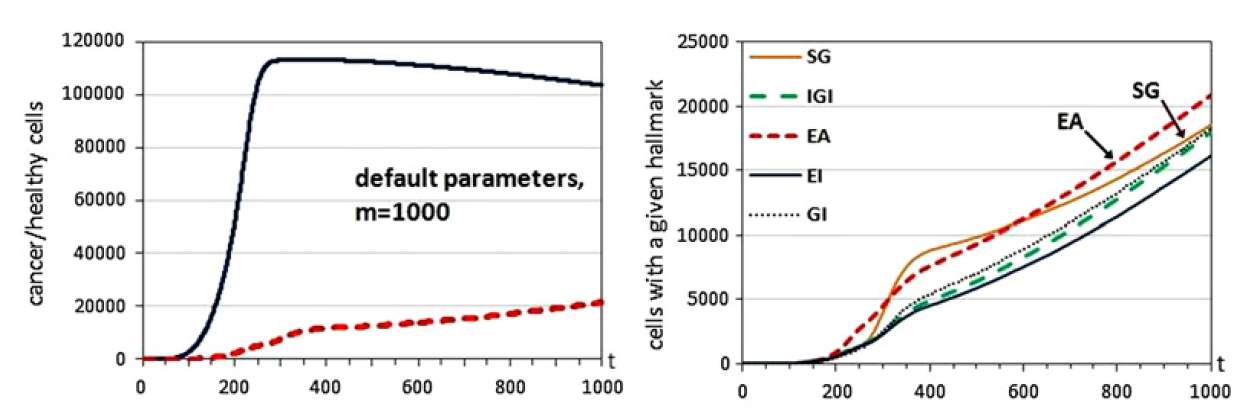
\includegraphics[scale=0.6]{figures/experiments/exp2}
\caption{Resultados obtenidos por los autores para el experimento con $m=1,000$.}
\end{figure}

\subsection{Experimento 3: Tasa de mutación base igual a 100}

En este tercer y último experimento de este tipo, los autores obtienen cambios relevantes frente a los dos
experimentos anteriores.

En primer lugar, el número de células cancerosas pronto supera a las células sanas, e incluso,
a lo largo de las iteraciones terminan, las células cancerosas, representando casi la totalidad de
la rejilla. Esto se explica por la mayor probabilidad de aparición de mutaciones durante la mitosis, en
este caso, la tasa de mutación base es de $m=100$.

En segundo lugar, en cuanto a marcadores, ocurren todos los marcadores con un comportamiento similar,
tomando ventaja, pero muy levemente, los marcadores $EA$ e $IGI$. La principal diferencia en este punto es
la presencia del marcador $IGI$, el cual, tiene mayor presencia que otros. El marcador $SG$ no toma ventaja en
este punto, como si lo hacía en los dos experimentos anteriores.

El marcador $EA$ siempre está presente y cobra un papel fundamental, ya que, permite la proliferación
de células cancerosas debido a que supone que la célula con dicho marcador puede evadir la muerte
celular programada.

\begin{figure}[h]
\centering
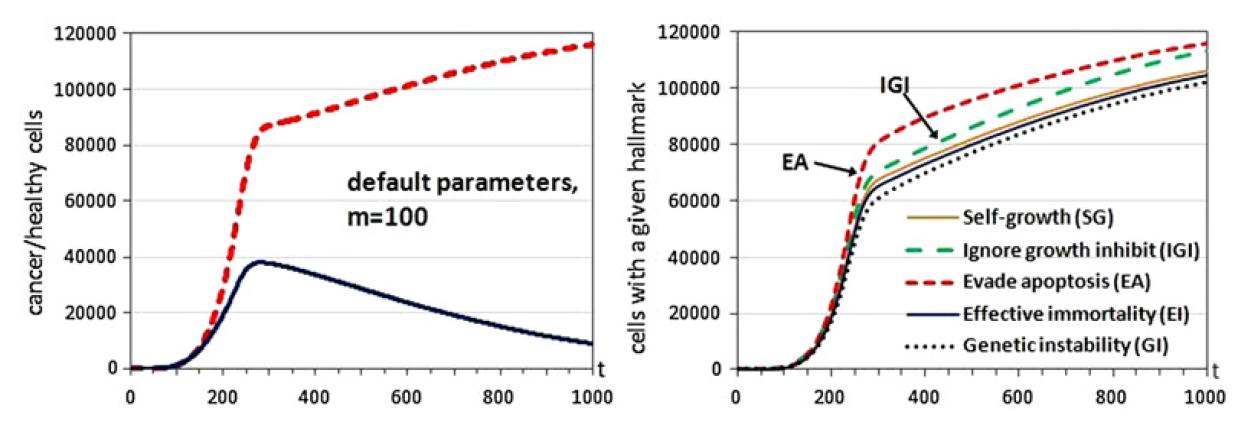
\includegraphics[scale=0.6]{figures/experiments/exp3}
\caption{Resultados obtenidos por los autores para el experimento con $m=100$.}
\end{figure}

\section{Influencia del resto de parámetros}

Los autores realizan un segundo experimento con el objetivo de observar los efectos
que tienen el resto de parámetros sobre la simulación. Para ello, varían los parámetros de
la simulación, como se puede observar en la siguiente tabla:

\begin{table}[h!]
  \centering
  \caption{Valores de los parámetros.}
  \label{tab:table1}
  \begin{tabular}{ccc}
    \toprule
    Nombre & Símbolo & Valor\\
    \midrule
    Tasa de mutación base & m & 100.000\\
    Tamaño del telómero & tl & 35\\
    Muerte por daño genético & e & 20\\
    Factor de incremento de tasa de mutación base & i & 100\\
    Muerte de un vecino & g & 10\\
    Muerte aleatoria & a & 400\\
    \bottomrule
  \end{tabular}
\end{table}

Se observa un comportamiento bastante representativo, por ejemplo, un menor valor
para el número de iteraciones implica menos eventos mitóticos en las células sanas, y
un menor valor del parámetros $a$ facilita la aparición de sitios vacacntes que
quedan disponibles para la propagación de células cancerosas, en conexión con una
mayor probabilidad de reemplazar a un vecino para realizar la mitósis (parámetros $g$).

En la gráfica de evolución de los marcadores se observa que en este caso el marcador
dominante es $EI$. En este caso, se realizan $5000$ iteraciones. El marcador $EI$ implica
la progresión de estas células debido a que evitan la muerte por agotamiento del telómero.
En la simulación, por contra, tener un telómero más corto implica tener menos oportunidades de división, como
ocurre con la célula inicial del centro de la rejilla.

El resto de marcadores aparecen más tarde en la simulación. El siguiente marcador en hacer
presencia es $EA$, lo cual permite a las células evadir la muerte celular programada. Este marcador
también favorece la proliferación del cáncer, por tanto, toma cada vez más ventaja. El marcador
$SG$ aparece algo más tarde que los anteriores y permite proliferar al cancer
fuera del límite reproductivo, por tanto, alcanza un límite y se mantiene estable.

El último marcador en aparecer es $IGI$. No prolifera rápidamente debido a no disponer
de espacio vacante para realizar la división.

\begin{figure}[h]
\centering
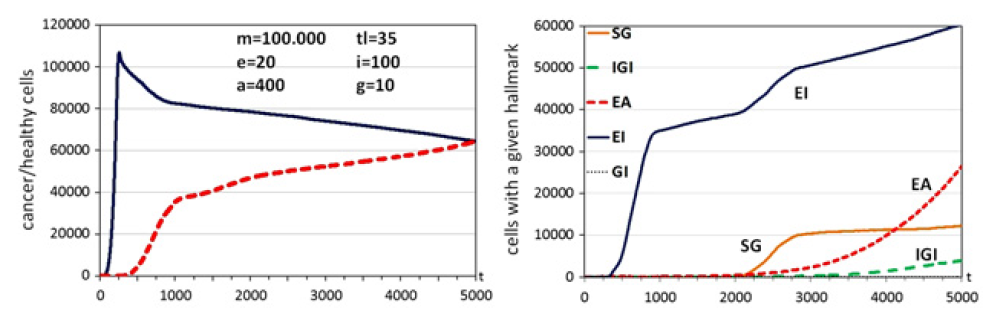
\includegraphics[scale=0.8]{figures/experiments/exp4}
\caption{Resultado de la simulación para comprobar la influencia del resto de parámetros.}
\end{figure}

\section{Influencia de parámetros con rejilla completa de células sanas}

En este caso, se parte con una rejilla completa de células sanas. En cuanto a los parámetros,
se utilizan los mismos que en la sección anterior.

Se realizan diferentes estrategias en cuanto al número de iteraciones, desde $8000$ iteraciones
hasta $100000$ iteraciones, es decir, la simulación se corresponde con una equivalencia temporal
de $2.3$ años y $29.7$ años respectivamente.

Completar.

\begin{figure}[h]
\centering
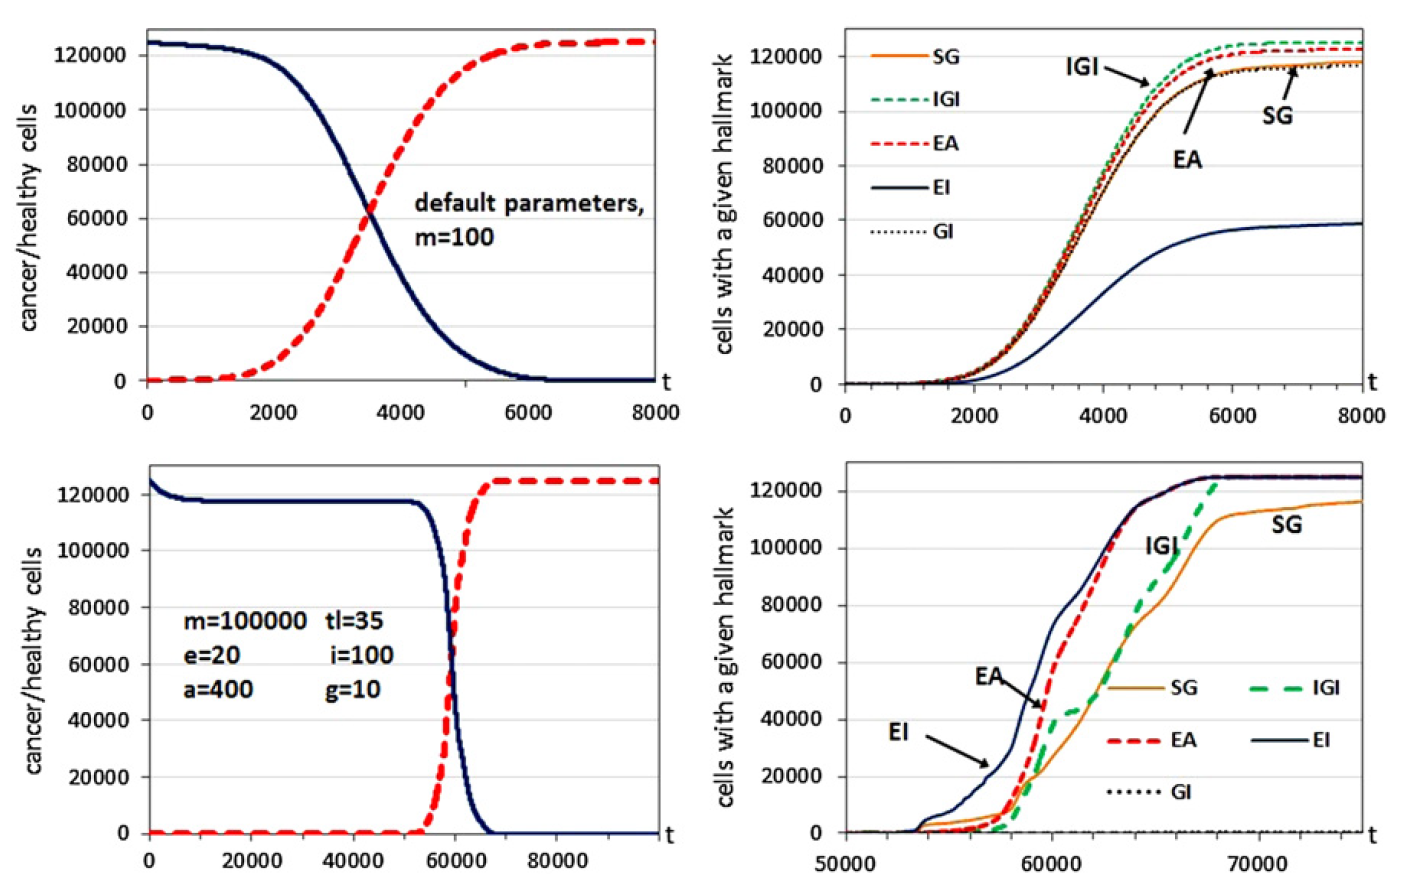
\includegraphics[scale=0.5]{figures/experiments/exp5}
\caption{Completar.}
\end{figure}

\section{Relevancia de los marcadores}

En este caso, los autores intentan responder a la siguiente pregunta: \textit{¿Cuál sería
el comportamiento emergente si algún marcador no estuviera presente y no aplicaran
sus efectos?}.

Conocer el efecto de cada marcador en el comportamiento emergente para crecimiento de tumores
puede resultar útil para mejorar las terapias contra el cáncer.

En su estudio, los autores encuentran el marcador $EA$ o de evasión de apoptosis como el más
relevante de todos, debido a que se reduce drásticamente el número de células cancerígenas.
Tras él, los siguientes marcadores más relevantes por orden son $GI$ o de inestabilidad genética y,
a continuación, $IGI$ o inhibición de señal de parada de crecimiento. Esto se debe a, en el caso
del marcador $GI$, se reducen las posibilidades de adquirir una mutación. Respecto al marcador $IGI$,
esto se debe a que cuando la rejilla no tiene espacio libre, sobre todo con células sanas, se reduce
la probabilidad de, para realizar la división, una célula mate a un vecino para conseguir espacio.

Completar.

\begin{figure}[h]
\centering
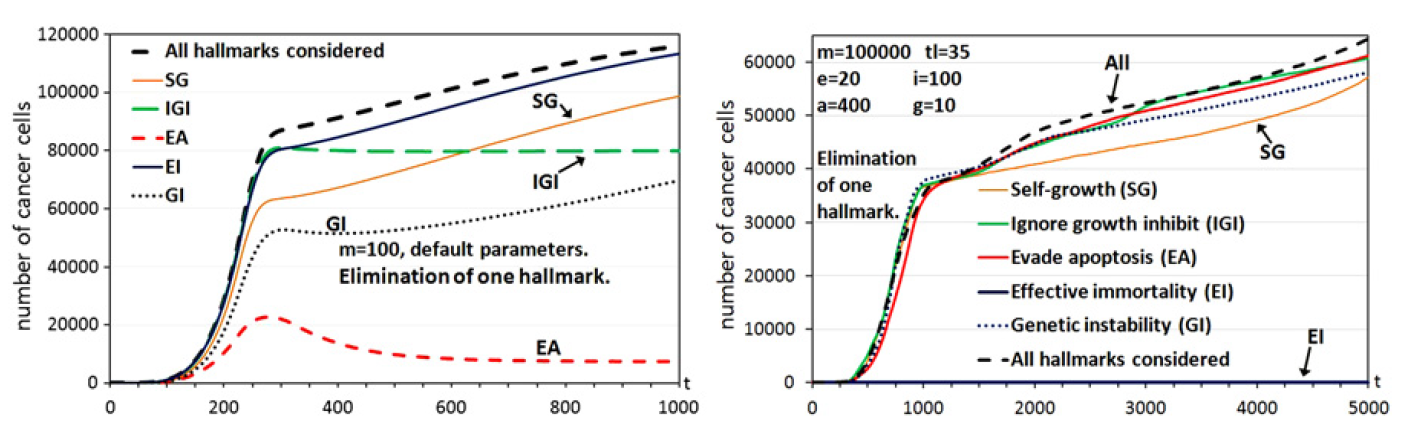
\includegraphics[scale=0.5]{figures/experiments/exp6}
\caption{Completar.}
\end{figure}

\section{Comportamiento de las transiciones}

El objetivo es estudiar el comportamiento de las transiciones cuando un agente actua contra las células cancerosas.
En este caso, la simulación comienza con la rejilla completa de células cancerosas, y se supone una terapia
perfecta, en el sentido que la droga, en este caso, actúa sólo contra las células cancerosas.

Completar.

\begin{figure}[h]
\centering
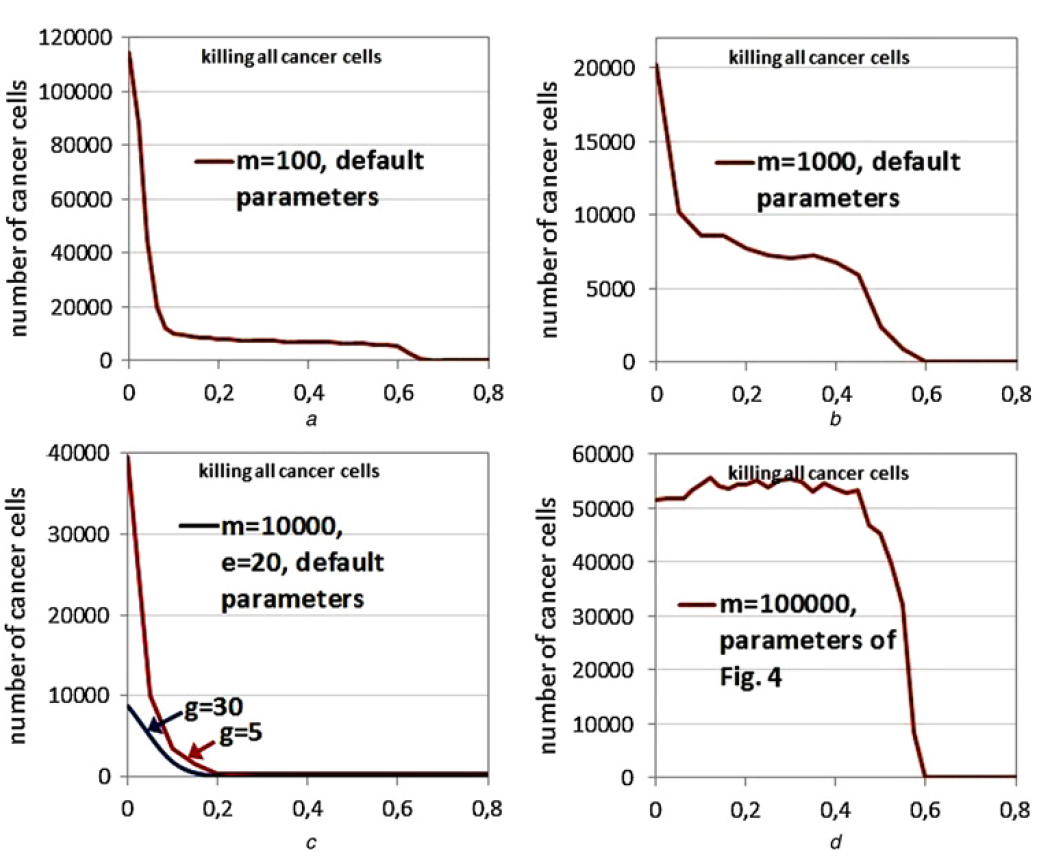
\includegraphics[scale=0.7]{figures/experiments/exp7}
\caption{Completar.}
\end{figure}

\begin{figure}[h]
\centering
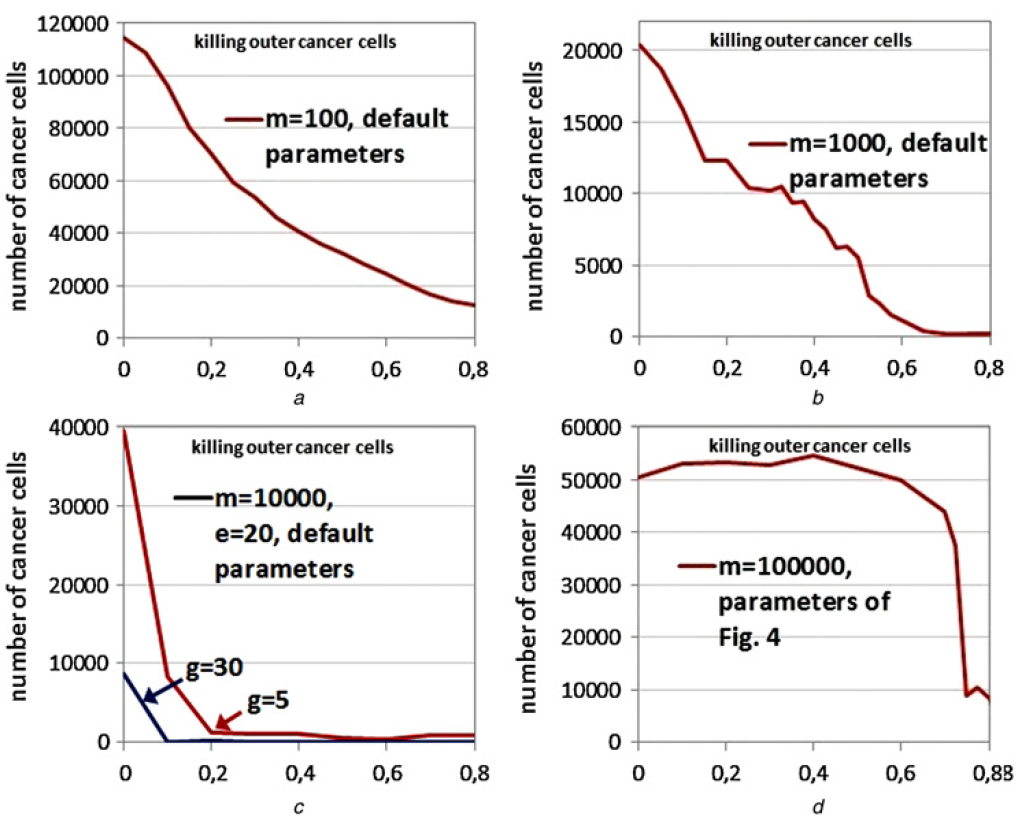
\includegraphics[scale=0.7]{figures/experiments/exp8}
\caption{Completar.}
\end{figure}
